\documentclass[transmag]{IEEEtran}
\usepackage{latexsym}
\usepackage{graphicx}
\usepackage{amsfonts,amssymb,amsmath}
\usepackage{hyperref}
\graphicspath{ {./images/} }
\renewcommand\IEEEkeywordsname{Keywords}
\usepackage{pdfpages}
\def\BibTeX{{\rm B\kern-.05em{\sc i\kern-.025em b}\kern-.08em T\kern-.1667em\lower.7ex\hbox{E}\kern-.125emX}}
\usepackage{float}
\usepackage{aliascnt}
\newaliascnt{eqfloat}{equation}
\newfloat{eqfloat}{h}{eqflts}
\floatname{eqfloat}{Equation}
\usepackage{cancel}
\usepackage{listings}
\usepackage{xcolor}

\definecolor{codegreen}{rgb}{0,0.6,0}
\definecolor{codegray}{rgb}{0.5,0.5,0.5}
\definecolor{codepurple}{rgb}{0.58,0,0.82}
\definecolor{backcolour}{rgb}{0.95,0.95,0.92}

\lstdefinestyle{mystyle}{
  %  backgroundcolor=\color{backcolour},   
    commentstyle=\color{codegreen},
    keywordstyle=\color{magenta},
    numberstyle=\tiny\color{codegray},
    stringstyle=\color{codepurple},
    basicstyle=\ttfamily\footnotesize,
    breakatwhitespace=false,         
    breaklines=true,                 
    captionpos=b,                    
    keepspaces=true,                 
    numbers=left,                    
    numbersep=5pt,                  
    showspaces=false,                
    showstringspaces=false,
    showtabs=false,                  
    tabsize=2
}

\lstset{style=mystyle}

\begin{document}

\title{\textsc{Robot Manipulator Design Assignment}}

\clearpage\thispagestyle{empty}

\author{Souto T.L.

\\
\\
\\

\begin{centering}
\vspace{20mm}

\includegraphics[scale=0.25]{massey-png}
\end{centering}



\thanks{This paper is a Individual design Project and It is part of the second assignment of the course Master of engineering - Mechatronics at Massey university, Auckland.

A GitHub repository with all the files used in this project is available \textcolor{blue}{\href{https://github.com/ThiagoSoutoGit/Robotic-Manipulator-Files}{here}}. 

Thiago Lima Souto is a student register under the number 19044686 at Massey university. Questions, comments or communications can be addressed via email \color{blue}\href{mailto:thiago.souto@yahoo.com.br}{thiago.souto@yahoo.com.br}
}}




\IEEEtitleabstractindextext{\begin{abstract}
In this project a mechatronic system is developed, this system is composed of a mechanical, a pneumatic and an electrical sub-systems. Ultrasonic sensors and microcontrollers are used to achieve the goal of distributing tennis balls on a basic packing system. 
The design was developed using tools like Proteus for the control and sensors, solidworks for the system mechanics and the Arduino IDE to program the microcontroller.


\end{abstract}



\begin{IEEEkeywords}
Mechatronic systems, pneumatics, ultrasonic sensors 
\end{IEEEkeywords}
}

\maketitle
\thispagestyle{empty}

\clearpage
\newpage

\clearpage\thispagestyle{empty}
\onecolumn

\tableofcontents

%\listoffigures

\lstlistoflistings

\clearpage
\newpage

\twocolumn




%\onecolumn



\section{INTRODUCTION}

 The main objective of this report is to design a mechatronic system capable of uniformly distribute tennis balls from a hopper onto a production line using pneumatics. This system shall be composed of a electrical, mechanical and software sub-systems in order to practice such skills.
 
 To accomplish this objective a system composed basically by one pneumatic actuator, a motor, two ultrasonic sensor and the mechanical system that integrates the hopper to the production line was designed.
 A pneumatic cylinder is used to push the tennis ball, that comes from the hopper and is unable to enter the production line because of a gate, into a rail that leads to a conveyor with a line of tennis ball's packages. 
 The first ultrasonic sensor is set to detect any object that is below 6 cm of distance and sends a signal to the solenoid valve that activate the cylinder, this step is required to verify if there is any balls coming from the surveyor.
 After the ball goes through the rail it ends up on the package and a second ultrasonic sensor, set to detect object at a distance below 20 cm, senses if the package is full and send a signal to the motor that pushes another package one step forward completing the cycle. 
 
 This report begins explaining why the use of pneumatics in conjunction with other systems, such is electrical actuation, is widely used. Then the actuation used on the model is discussed as well as the electronics and sensors. The simulation tools used are then explained and also how they interact with each other.
Finally the outcome of this project is discussed and the conclusions exposed.



\section{Methodology}

At this section of the report, for each aspect of the project, a small discussion  and the necessary explanations that will support the decisions made around pneumatics, actuation, electronic control and simulation, will be rendered. 
The intention is to, first, give a general view of the parts of the subject that will have an impact in what was used on the project. Second to explain why this was done. For example, on pneumatics, compressors and reservoirs are discussed and why they are not on simulations.

Also the tools and software used to achieve the results and how these results were achieved.

Finally, the relation of each part with the objectives of the report is exposed. Figures and listings will illustrate the explanation wherever necessary.

\subsection{Pneumatics}

In a pneumatic system normally air is drawn from the atmosphere via an air filter and raised to the system required pressure by an air compressor, which is normally driven by a AC motor. \cite{ref1} Because the air contains a significant amount of water vapour the air must be cooled and treated before being used. 

Pressurized air is then stored in a reservoir and can be released to the cylinder, without the reservoir the valve action could be slow, if the pressure was to be raised every time the valve was to be used.

The pneumatic systems may look complex and for small applications such as this demonstration project it is no feasible, although many factories produce compressed gas  at a central and distribute it on a air ring main to all places on the site, in a similar fashion as electricity or water.

The development of a pneumatic system will make possible, by studying small systems like this project to have a better idea on large scale plants and how they integrate their systems.

For a matter of convenience the pressure reservoir and compressor will be excluded of the simulations included in this report.




\subsection{Actuation}

The actuation systems are responsible for transforming the control system output into an action that will control the system \cite{ref2}, on this project solenoid valves are used to control the flow of air which will start the pneumatic cylinder. 
The pneumatic cylinder is an example of a linear actuator, it consists of a cylindrical tube along which a piston can slide. The cylinder used on the project is shown on Figure \ref{Cylinder}.

\begin{figure}[h]
\centerline{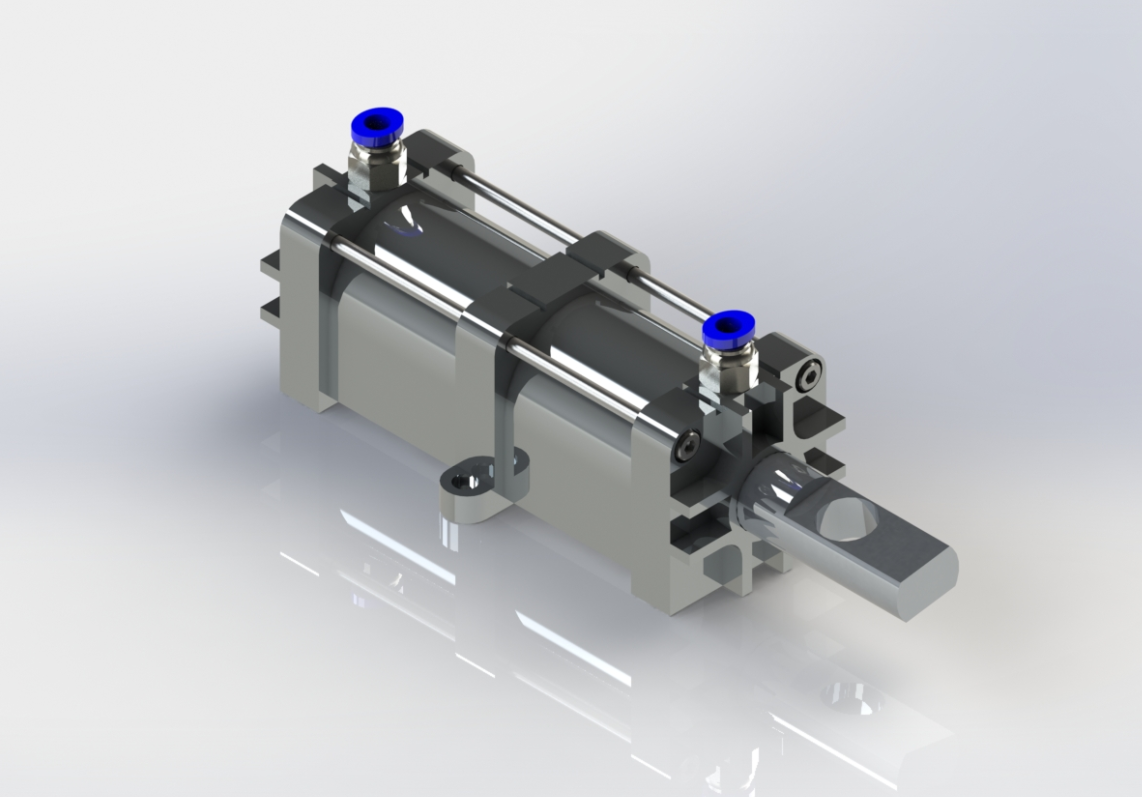
\includegraphics[width=3.5in]{./images/Cylinder}}
\caption{Cylinder \cite{ref2}\label{Cylinder}}
\end{figure}


To control the motor which will control the conveyor belt a relay is used, it is  represented by the LED at the electronic simulation, it works as a mechanical switch acting as the motor actuator.

Relays are widely used on control systems in conjunction with a transistor (Figure \ref{Relay}) to switch on the current through the solenoid to switch on the much larger current needed to switch on or off a final correction element such as a motor.\cite{ref2}

\begin{figure}[h]
\centerline{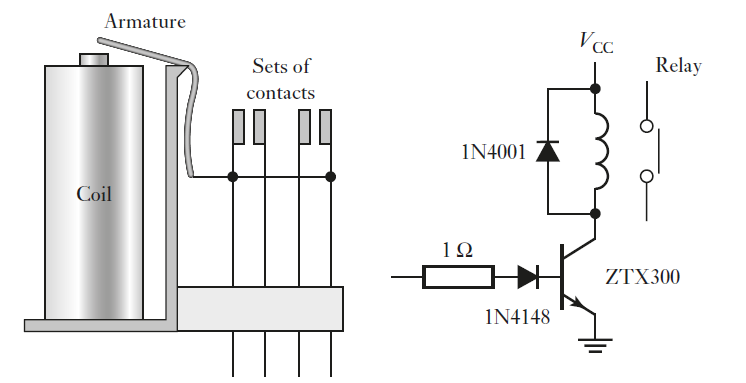
\includegraphics[width=3.5in]{./images/Relay}}
\caption{Relay with a transistor \cite{ref2}\label{Relay}}
\end{figure}

These are some of the various kinds of actuation systems, to know how to integrate them on pneumatic systems is crucial for modern operations. 





\subsection{Electronic system}

The electronic system is composed by two ultrasonic sensors, a LCD display, and a microcontroller. The LCD monitor displays the actual distance between the ultrasonic sensors and the subjects of measurement, there will be displayed $UT cm:$ for the first measurement and $UT cm2:$ for the second. This is necessary so the correct functioning of the system can be judged. 


\subsubsection{LCD display}

The LCD module used was a 16x2 very commonly used in embedded projects, because its cheap, available and easy to program. They are very common on calculators. It has 16 Columns and 2 Rows. So, it will have 32 characters in total and each character will be made of 5×8 Pixel Dots. \cite{ref4}

\begin{figure}[h]
\centerline{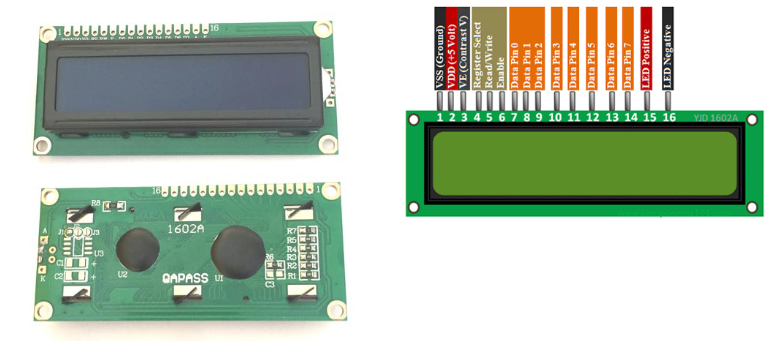
\includegraphics[width=3.5in]{./images/Display}}
\caption{16x2 Display\label{Display}}
\end{figure}

\subsubsection{Ultrasonic sensors}

An ultrasonic transducer transforms mechanical sound waves in electricity via a piezoelectric crystal. This crystal if cut on the x-axis has the property of changing size and shape when energy is applied, making the crystal vibrate and producing sound waves. The same occur at the reception of a sound wave , where the crystal receive the impact and produces energy. Figure \ref{Ultrasonic} illustrate how this can be done. \cite{ref6}

\begin{figure}
\centerline{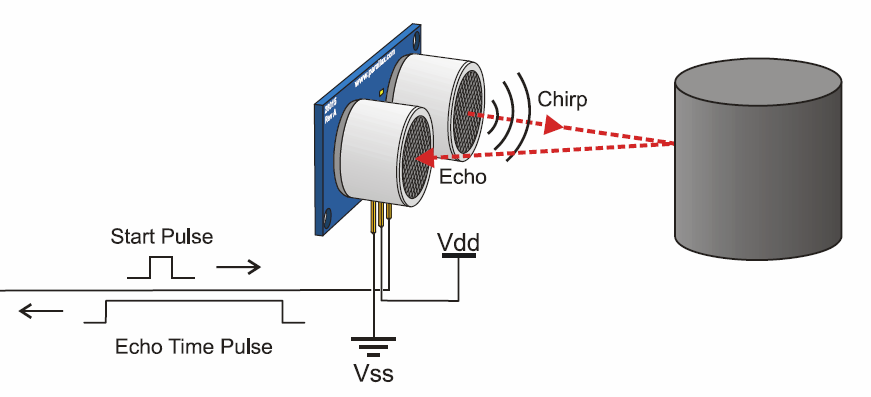
\includegraphics[width=3.5in]{./images/Ultrasonic}}
\caption{Ultrasonic Sensor\label{Ultrasonic}}
\end{figure}

This ultrasonic sensors can be used in quantity by the same microcontroller, as can be seen on Figure \ref{multiplesensors}, in this project only two were used.

\begin{figure}[h]
\centerline{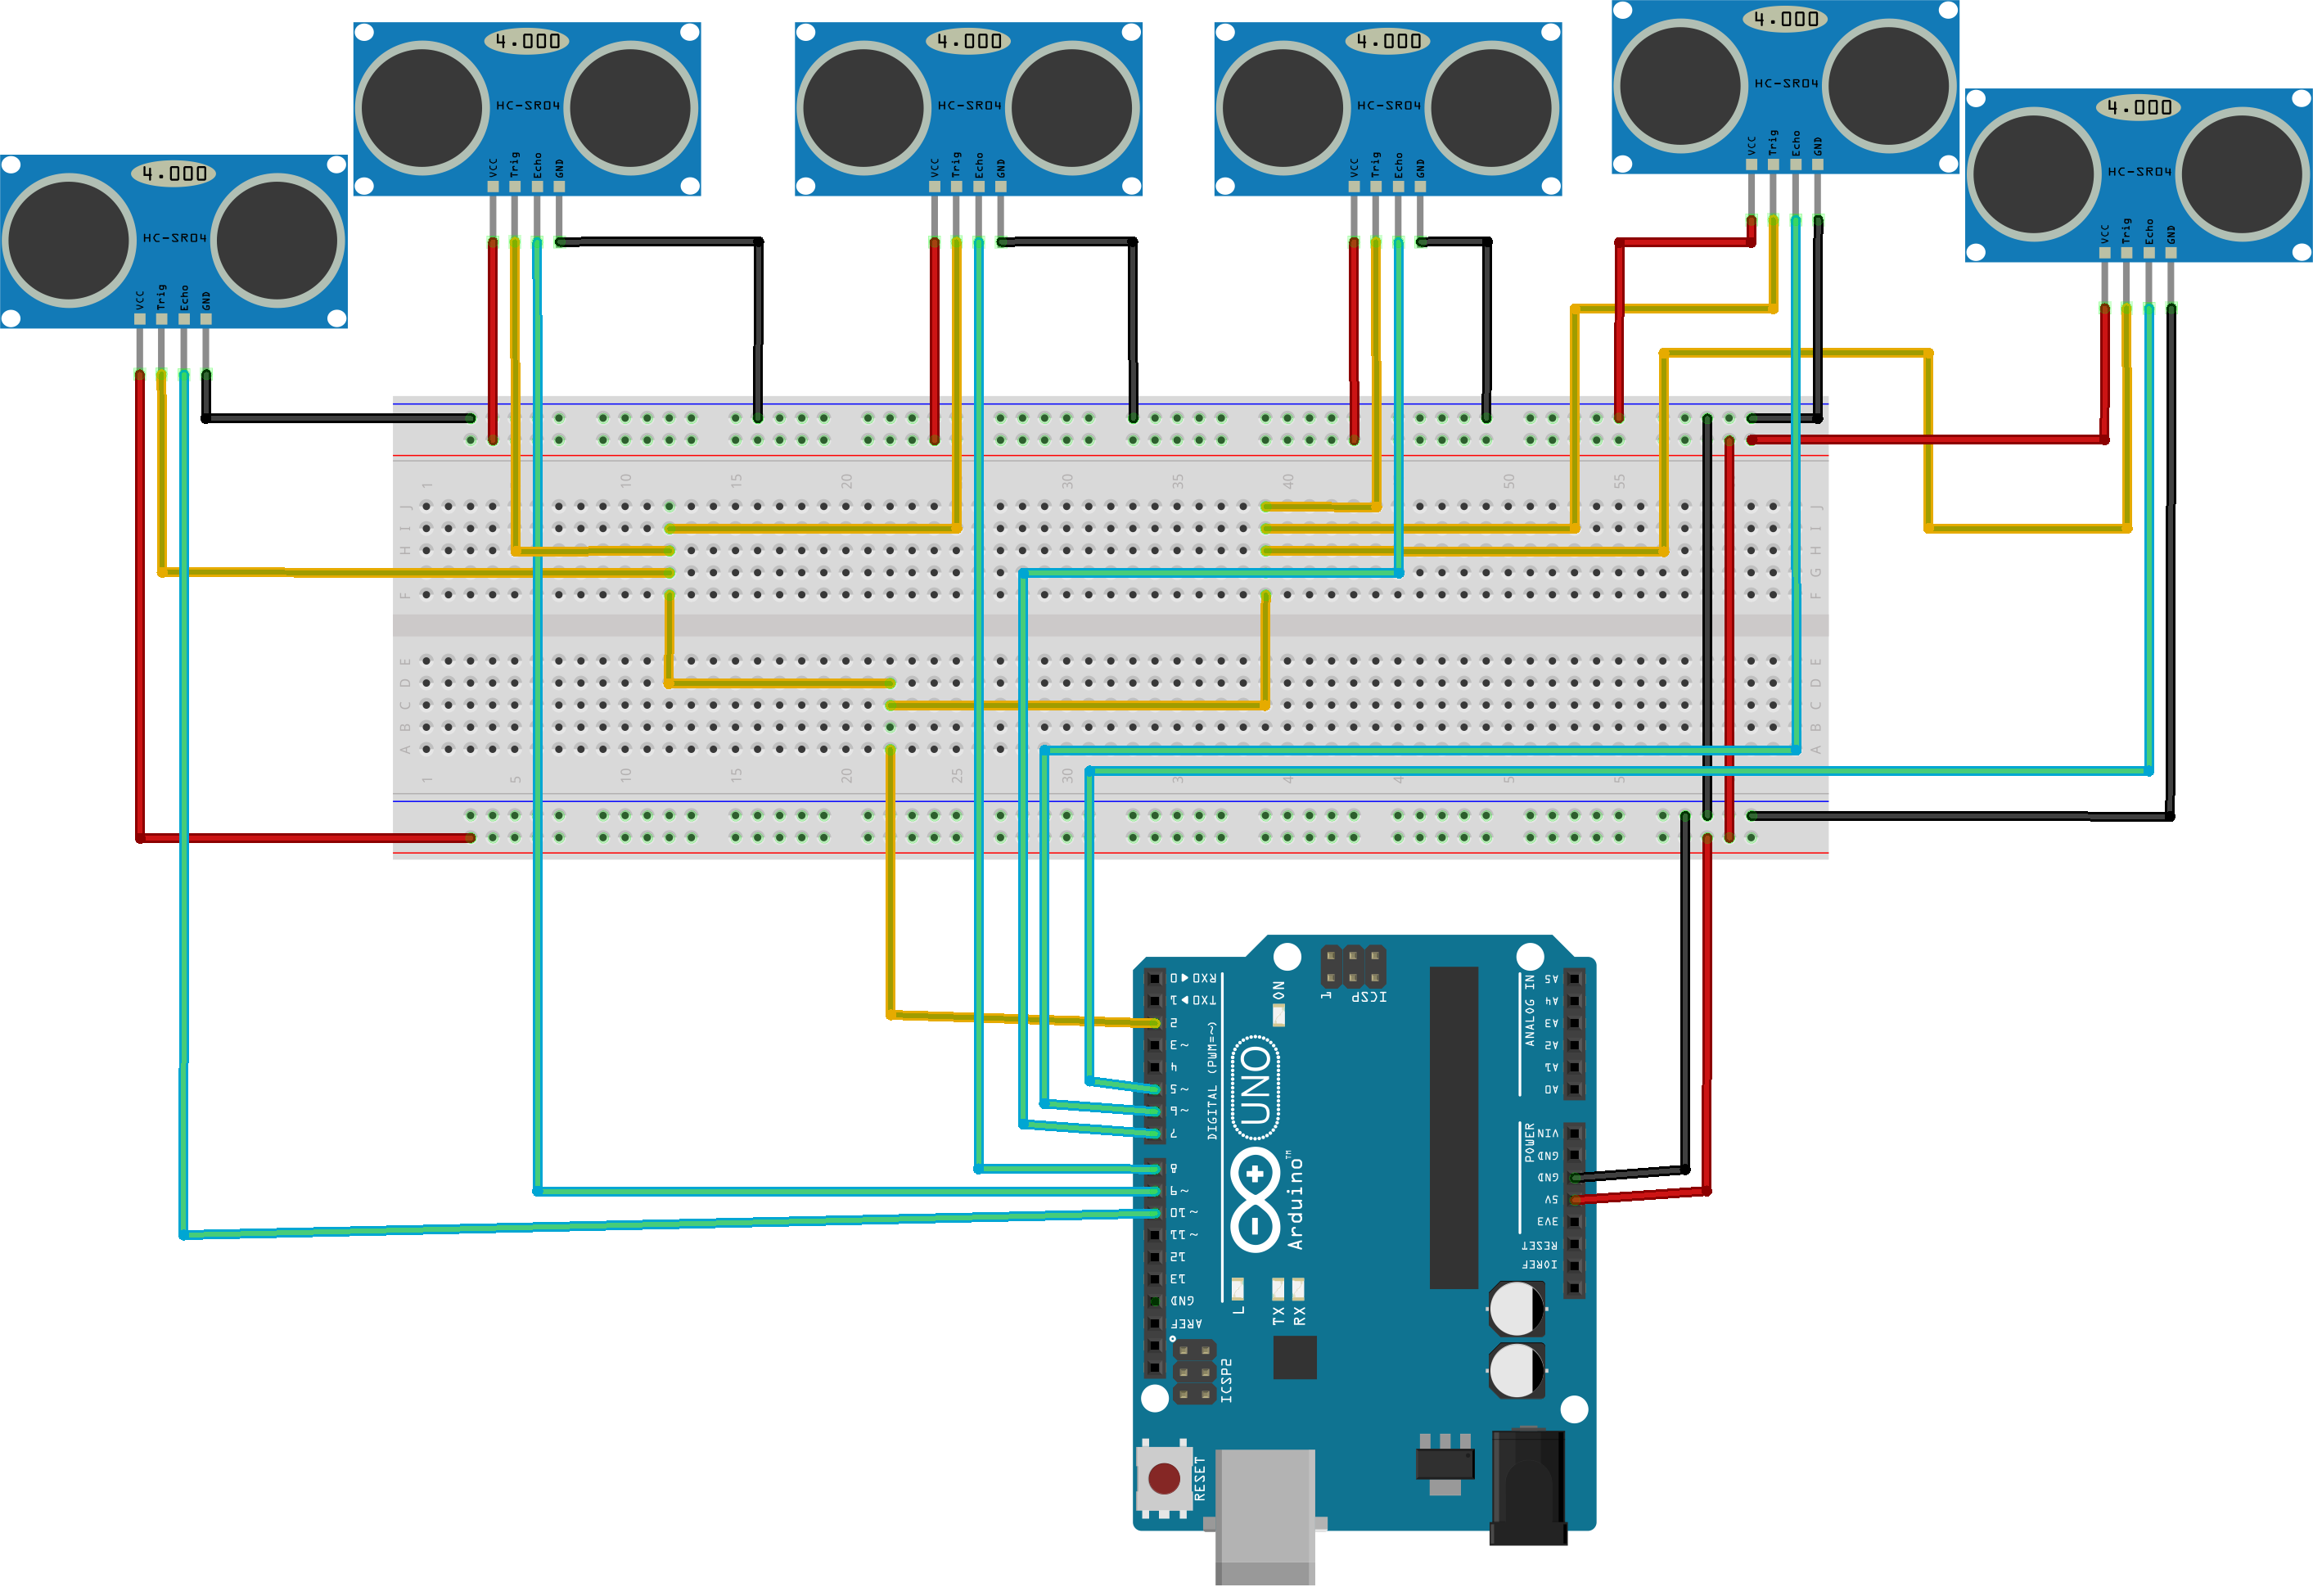
\includegraphics[width=3.5in]{./images/multiplesensors}}
\caption{Multiple sensors\label{multiplesensors}}
\end{figure}



\subsection{Microcontrollers}

A microcontroller is basically a a whole computer as a miniature. Different from the microprocessor that is the part of the system that process data, the microcontroller has memory, CPU, Digital pins for I/O (Input/Output). 
The microcontrollers used in this projects is the ATmega328P mounted on an Arduino Uno board. This microcontroller weights only 25g and have 1KB of EEPROM, 2KB of SRAM and 32 KB of flash memory. \cite{ref5}


\subsubsection{Control Methodology}

The control methodology consists, first, in verify if the there is a tennis ball in place, in front of the the first ultrasonic sensor, if affirmative the cylinder will push the ball down the rails and into the package, It will wait for one second and will verify again. In the case of no balls in front of the first ultrasonic sensor the system stops.

Then, as a second verification, using the second ultrasonic sensor the distance between the sensor and the inside of the package containing the balls is measured and if the distance is less than 20 cm, which means that there are three balls inside the package, a signal is sent to the motor the will roll the belt and place another empty package on the place. The motor works for 1 second, time necessary to put another pack in place and time enough for another ball to come if the hopper is not empty yet.


 
\section{Design Process}

The Design Process section is excellent. It discusses the employed design process, describing key stages and highlighting its advantages and disadvantages. It also discusses the process in relation to the assessment’s aims and objectives, and the defined specifications. Appropriate figures are used to effectively illustrate the design process.

The design process consisted of three main phases, first an ideation process and research. In this Phased a research around previous projects, interview with other students, literature review was first conducted as wells as discussions with the professors to understand the problem. Also in this phased a ideation process was conducted to realize what would the project be in a high level and what kind of tools would be the best for the purpose.
After the first phased was decided that a system with two ultrasonic sensors, a cylinder and a conveyor belt with a motor would be designed.

A second Phased consisted in making the electrical simulation of the control system using potentiometers to mock the ultrasonic response for the distance and to analyse the control system timing. The great advantage of these phase is to avoid errors when buying the real parts and making sure the system is working prior to irreversible decisions. In this phase is possible even to further the capabilities of the project, add features and improve the concept of the project. 


Once satisfied with the electronic design and control system a CAD model was developed to study the dynamics of the interactions between the parts of the mechanical design and well as to have the measurements for the implementation of the project in the future.

The disadvantage is that theoretical components are much closer to ideal situations then to the reality and some adjustments may be necessary in the case of implementation in the real world, specially involving motors and pressurized systems as in the case of this project. 

The use of more robust software and real specifications from vendors as well as environment modifications on the simulation can mitigate some of these problems but never at a level of total confidence. Although, for the present work the tools used were more than suitable.


\subsection{Electronic simulation}


Virtual Prototyping enables system testing before fabrication and electronic devices such as sensors and microcontrollers ca be simulated in specialized software such as Proteus, which has over 15 million parts designed and can accelerate the design process.

\subsubsection{Proteus}

The Proteus Design Suite is used across various industry sectors as a solution for professional PCB design and as a rapid prototyping tool for R$\&$D \cite{ref3}. This tool was chosen due to the easy of use and simulating capacity, as well as per the amount of parts available, including the ones o=used on the project.
With Proteus there is the possibility of importing the programming to the part and simulate accurately the results.

In order to simulate the ultrasonic sensors input, a potentiometer is connected to the ultrasonic sensor test and a DC generator is connected in one side and ground on the other side. 

The first ultrasonic sensor, connected on pins 8 and 9, receives a DC generator of $50 mV$ in order to simulate a distance below 6 cm stipulated. If a distance below 6 cm is detected then it means that there is a tennis ball waiting to be pushed thorough the gate to the conveyor and the cylinder is activated, as shown on Figure \ref{Proteus1}. 

\begin{figure}[h]
\centerline{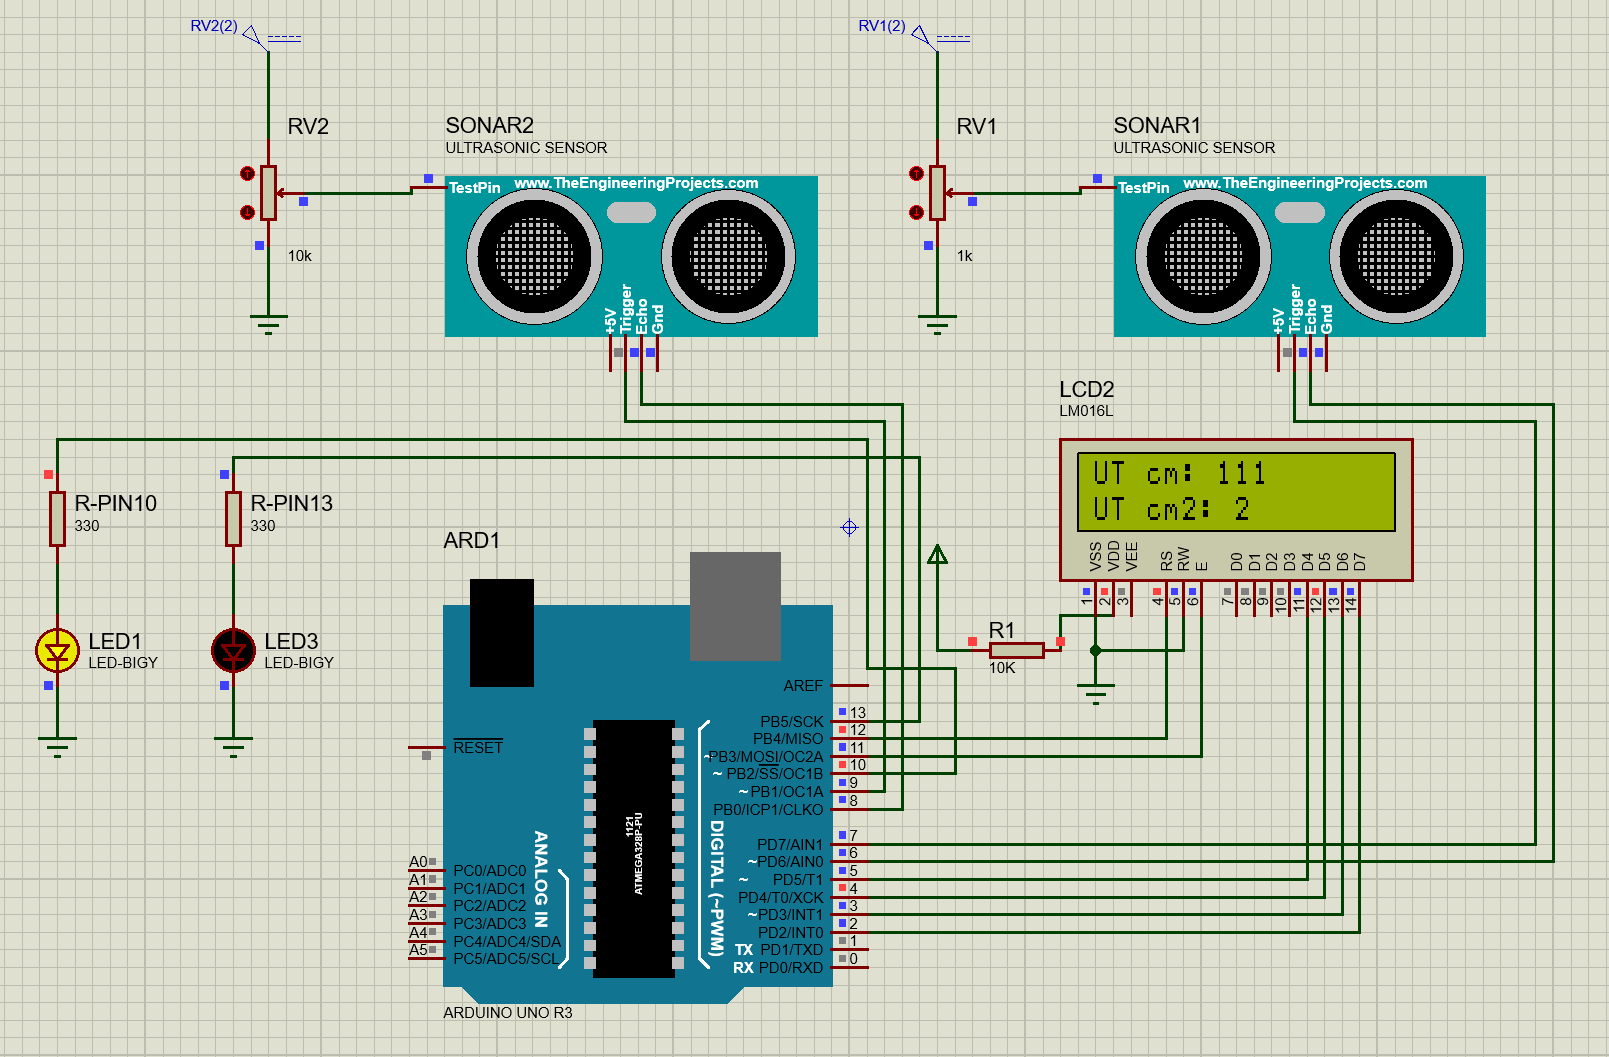
\includegraphics[width=3.5in]{./images/Proteus1}}
\caption{Simulation in Proteus - Sensor 2 below 6cm\label{Proteus1}}
\end{figure}

The second sensor receives a DC generator of $500 mV$ and simulates a 20 cm distance. It is located on top of the packing station and when there are three balls inside the pack it activates a motor that makes the conveyor belt roll a distance of one pack, and the full pack is projected forward while another one empty takes its place. Figure \ref{Proteus2} shows the system simulating a full pack being detected.

\begin{figure}[h]
\centerline{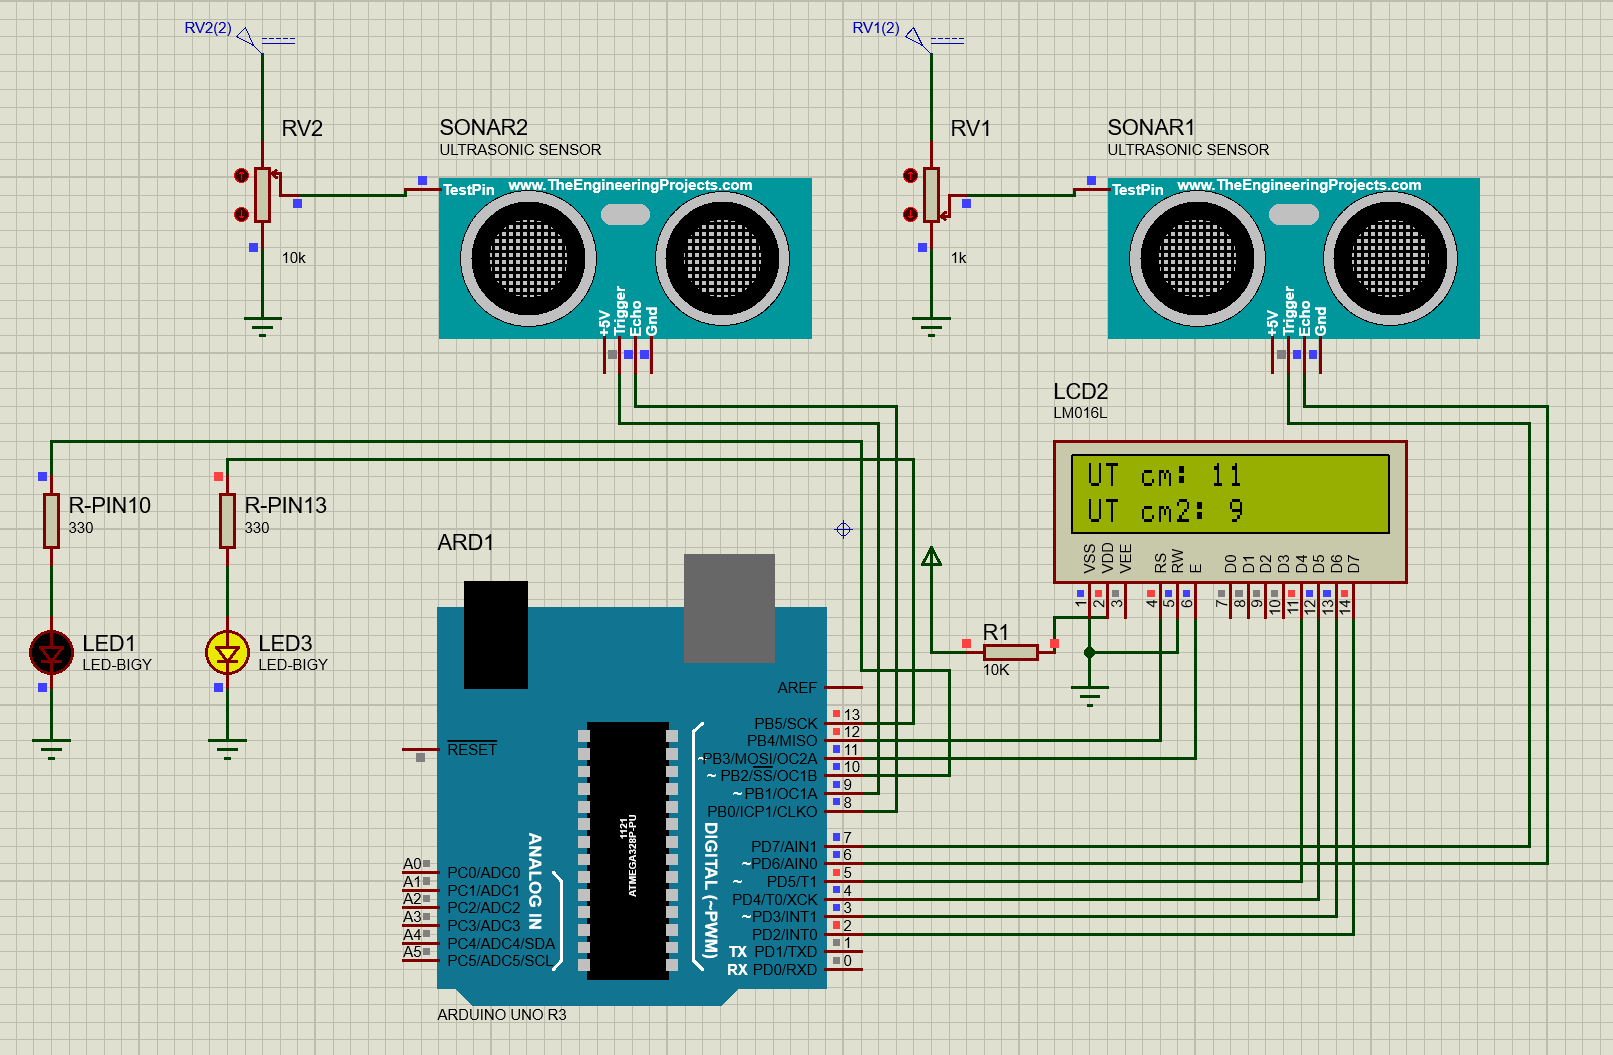
\includegraphics[width=3.5in]{./images/Proteus2}}
\caption{Simulation in Proteus - Sensor 1 below 20cm\label{Proteus2}}
\end{figure}


\subsection{Mechanical Simulation}

The mechanical design was made using Solidworks. There are many reasons to use this tool, its popularity results in a huge community of developers, amateurs and professionals that exchange experiences and solve problems. Solidworks have various modules that enable one to make physical simulations, animations and much more. An Overall view of the system is shown on Figure \ref{Line}.
On Figures \ref{FirstUT} and \ref{SecondtUT} is possible to see the position of the ultrasonic sensors.

\begin{figure}[h]
\centerline{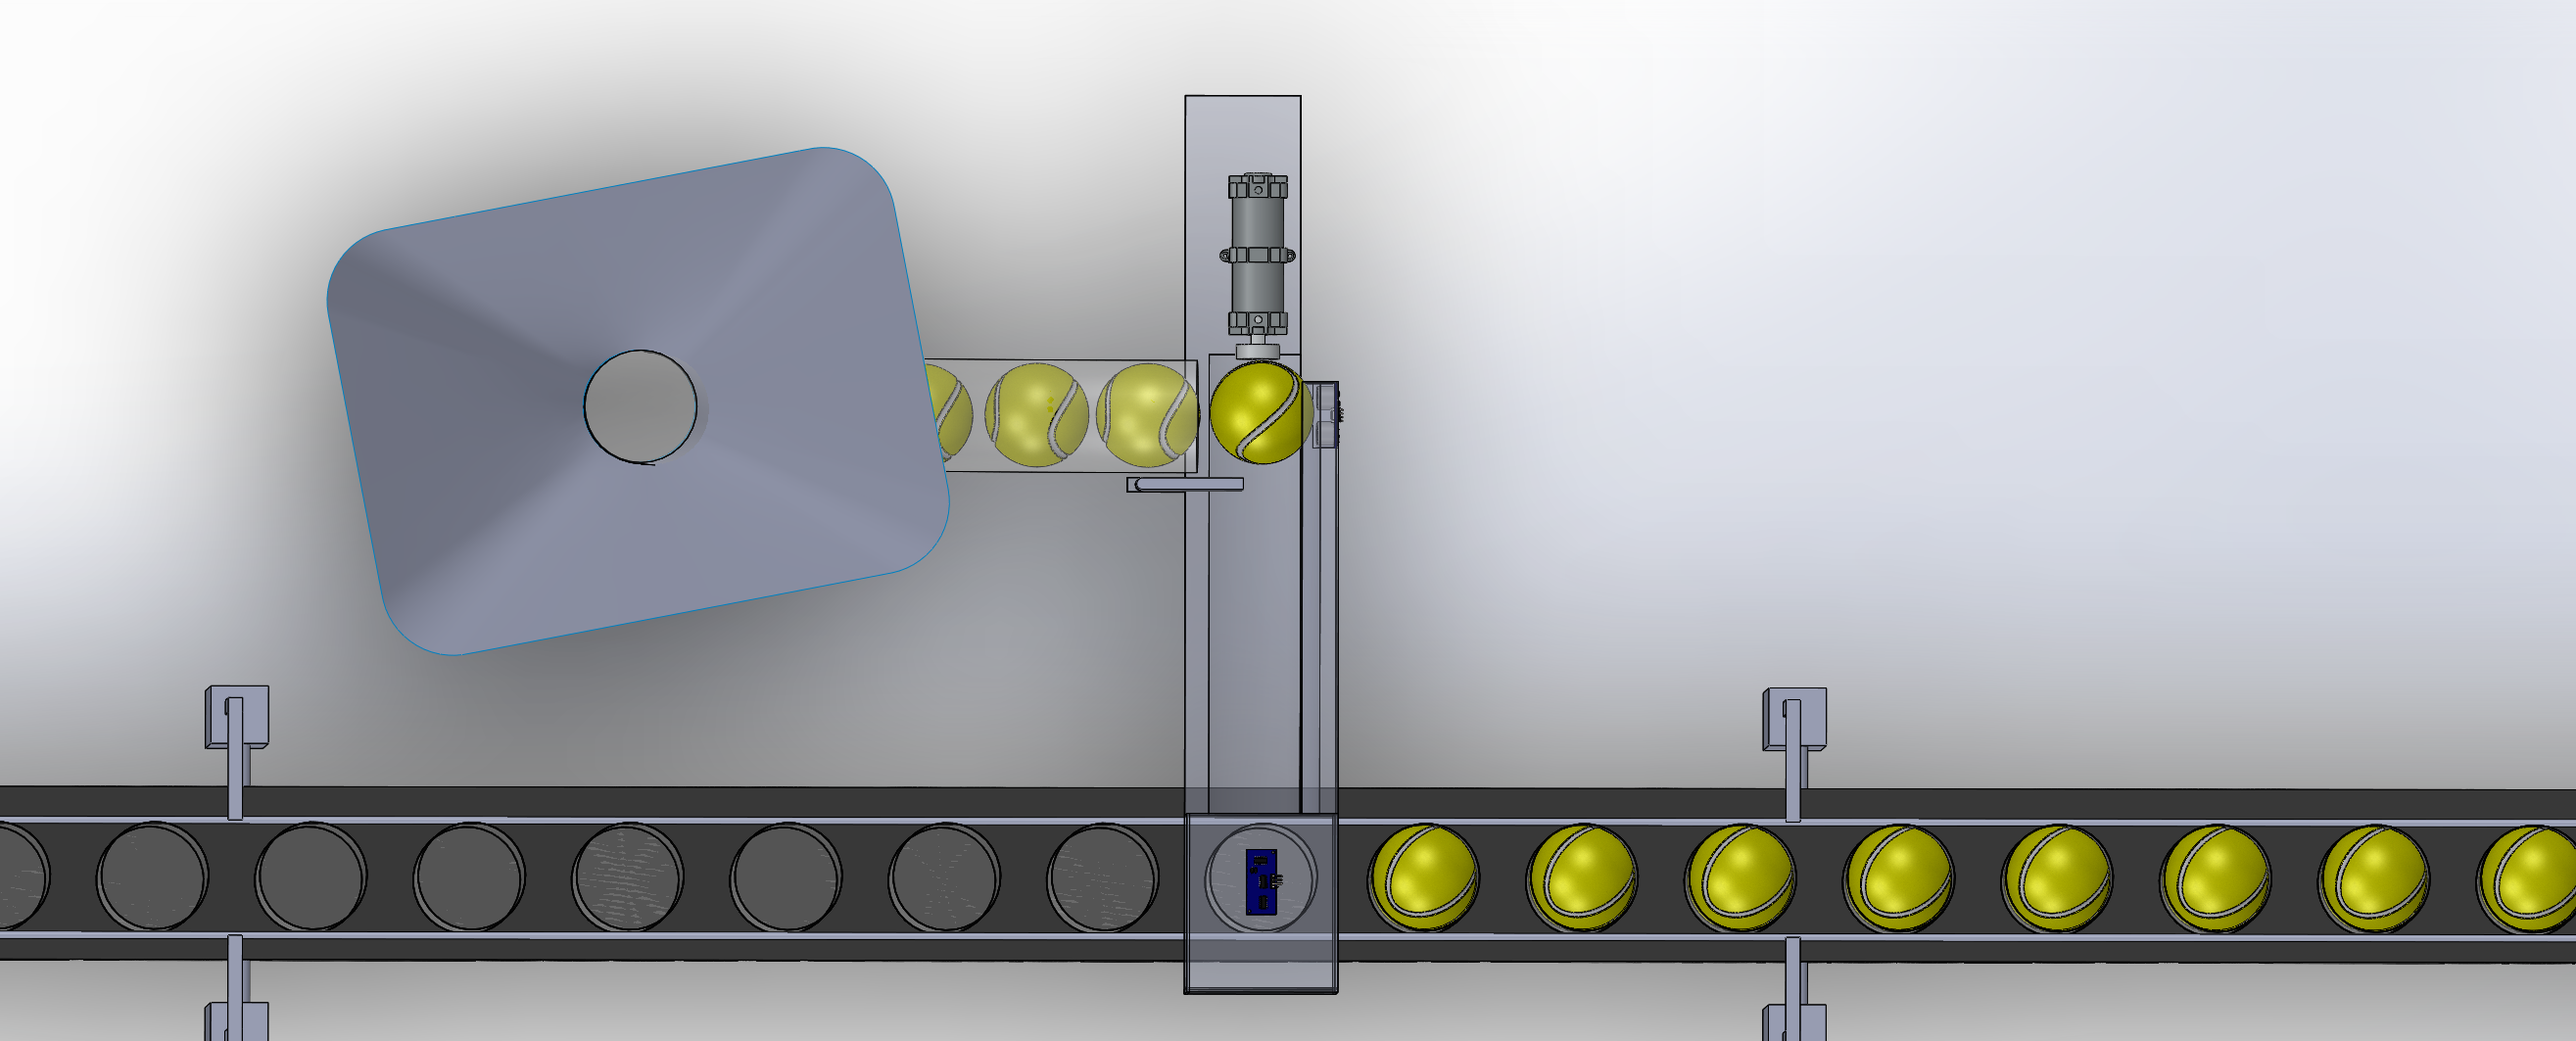
\includegraphics[width=3.5in]{./images/SecondUT}}
\caption{Sensor 2\label{SecondUT}}
\end{figure}

\begin{figure}[h]
\centerline{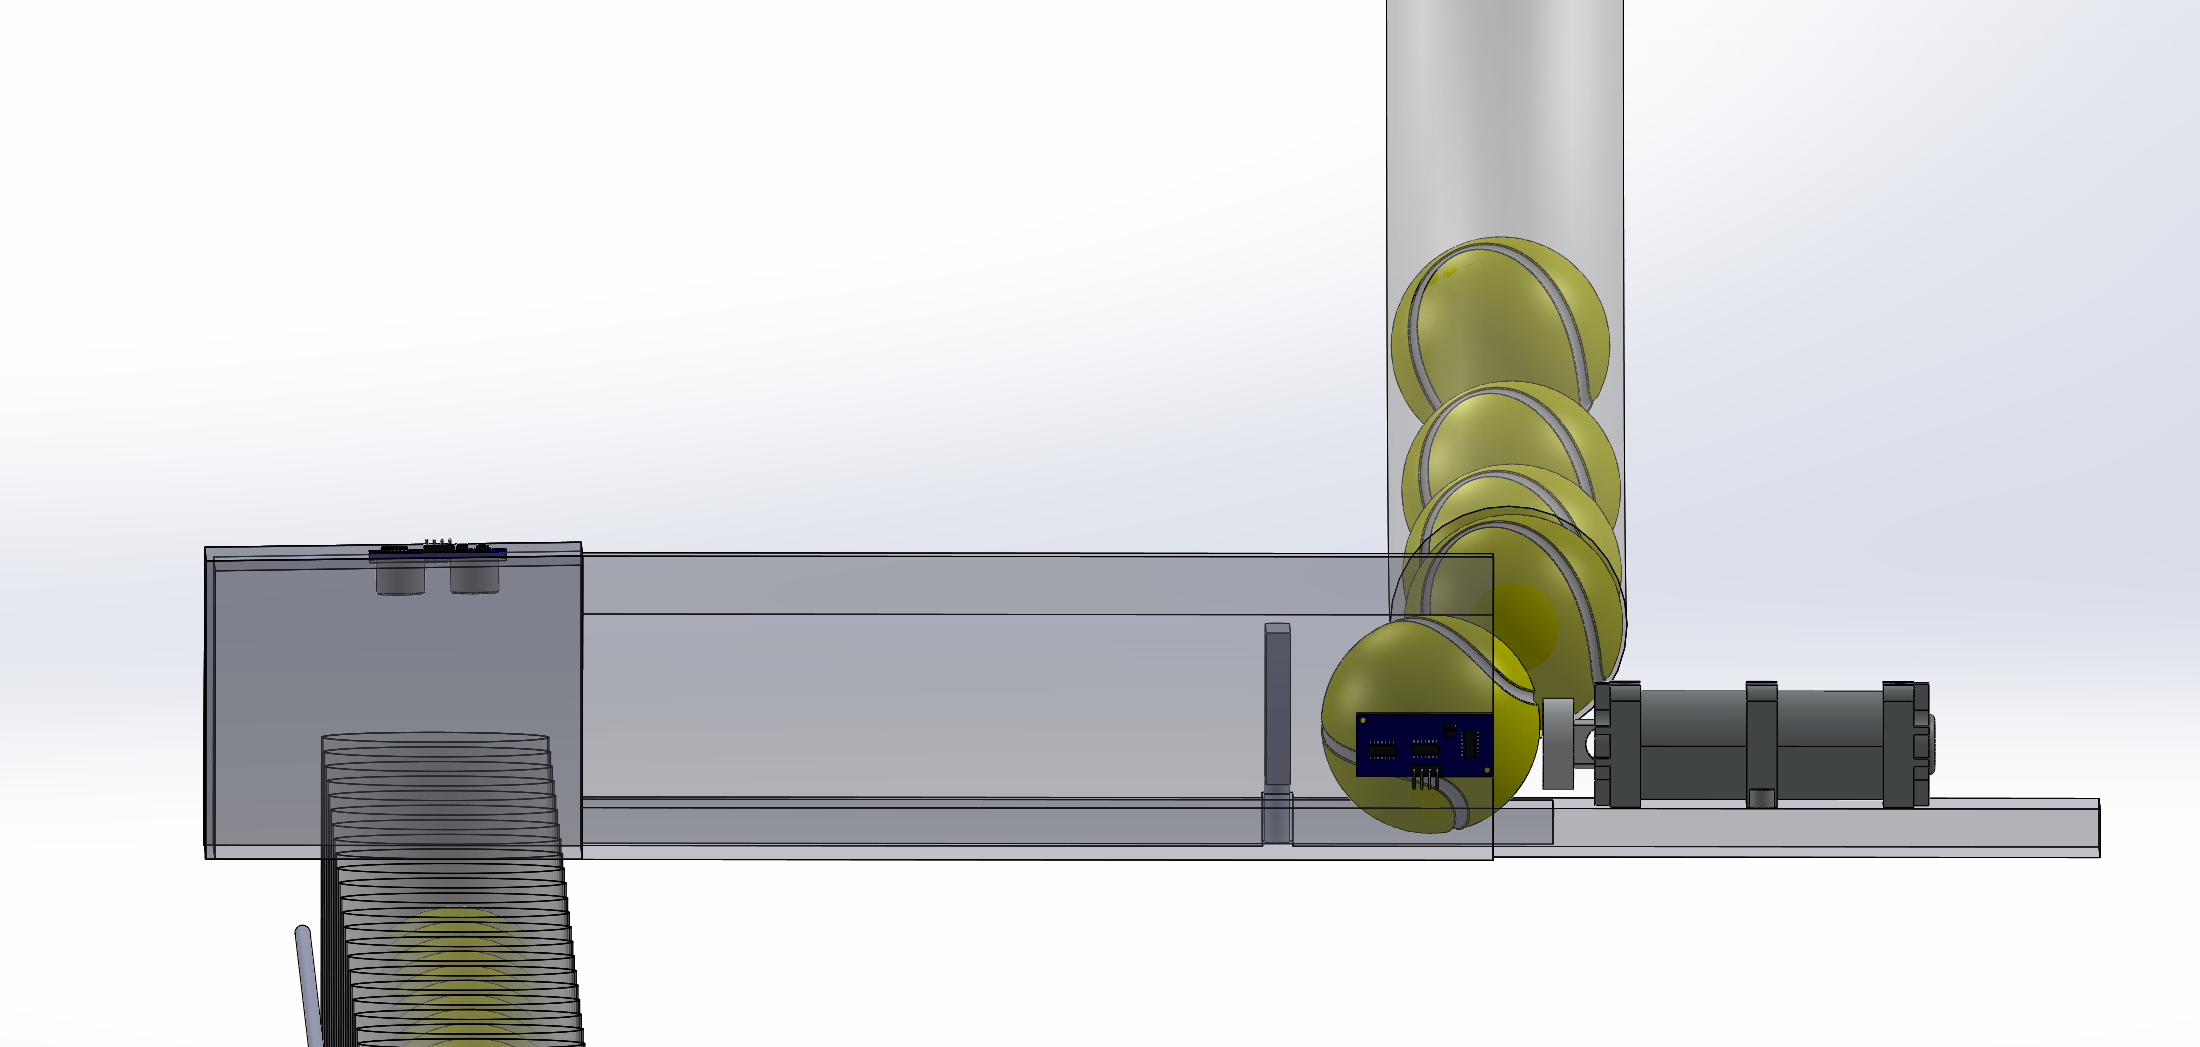
\includegraphics[width=3.5in]{./images/FirstUT}}
\caption{Sensor 1\label{FirstUT}}
\end{figure}

A view of the cylinder on Figure \ref{Line3} show a tennis ball being pushed by the gate and going at the production line's direction.

\begin{figure}[h]
\centerline{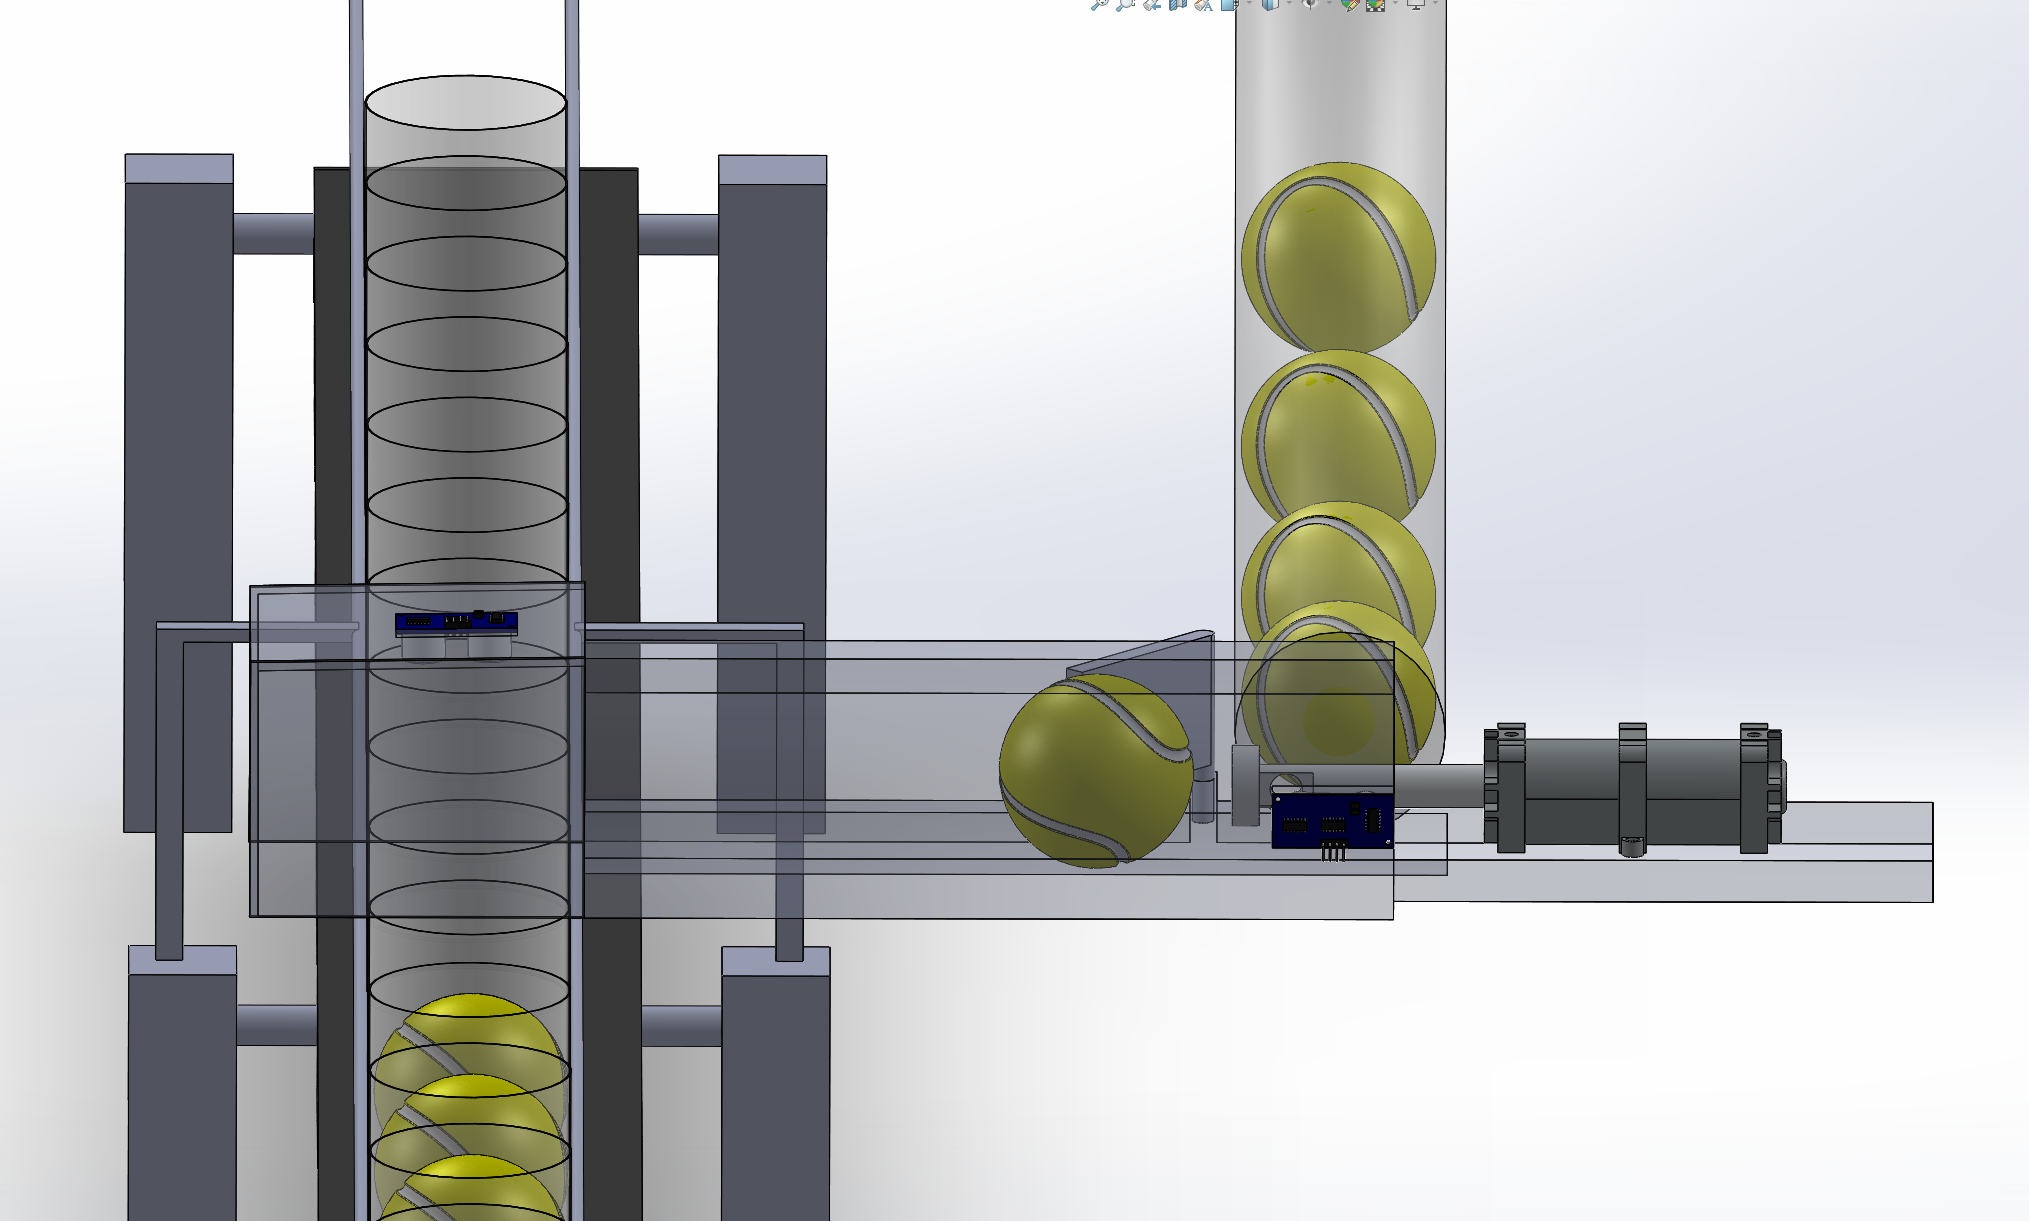
\includegraphics[width=3.5in]{./images/Line3}}
\caption{View of the cylinder\label{Line3}}
\end{figure}



\begin{figure*}
\centerline{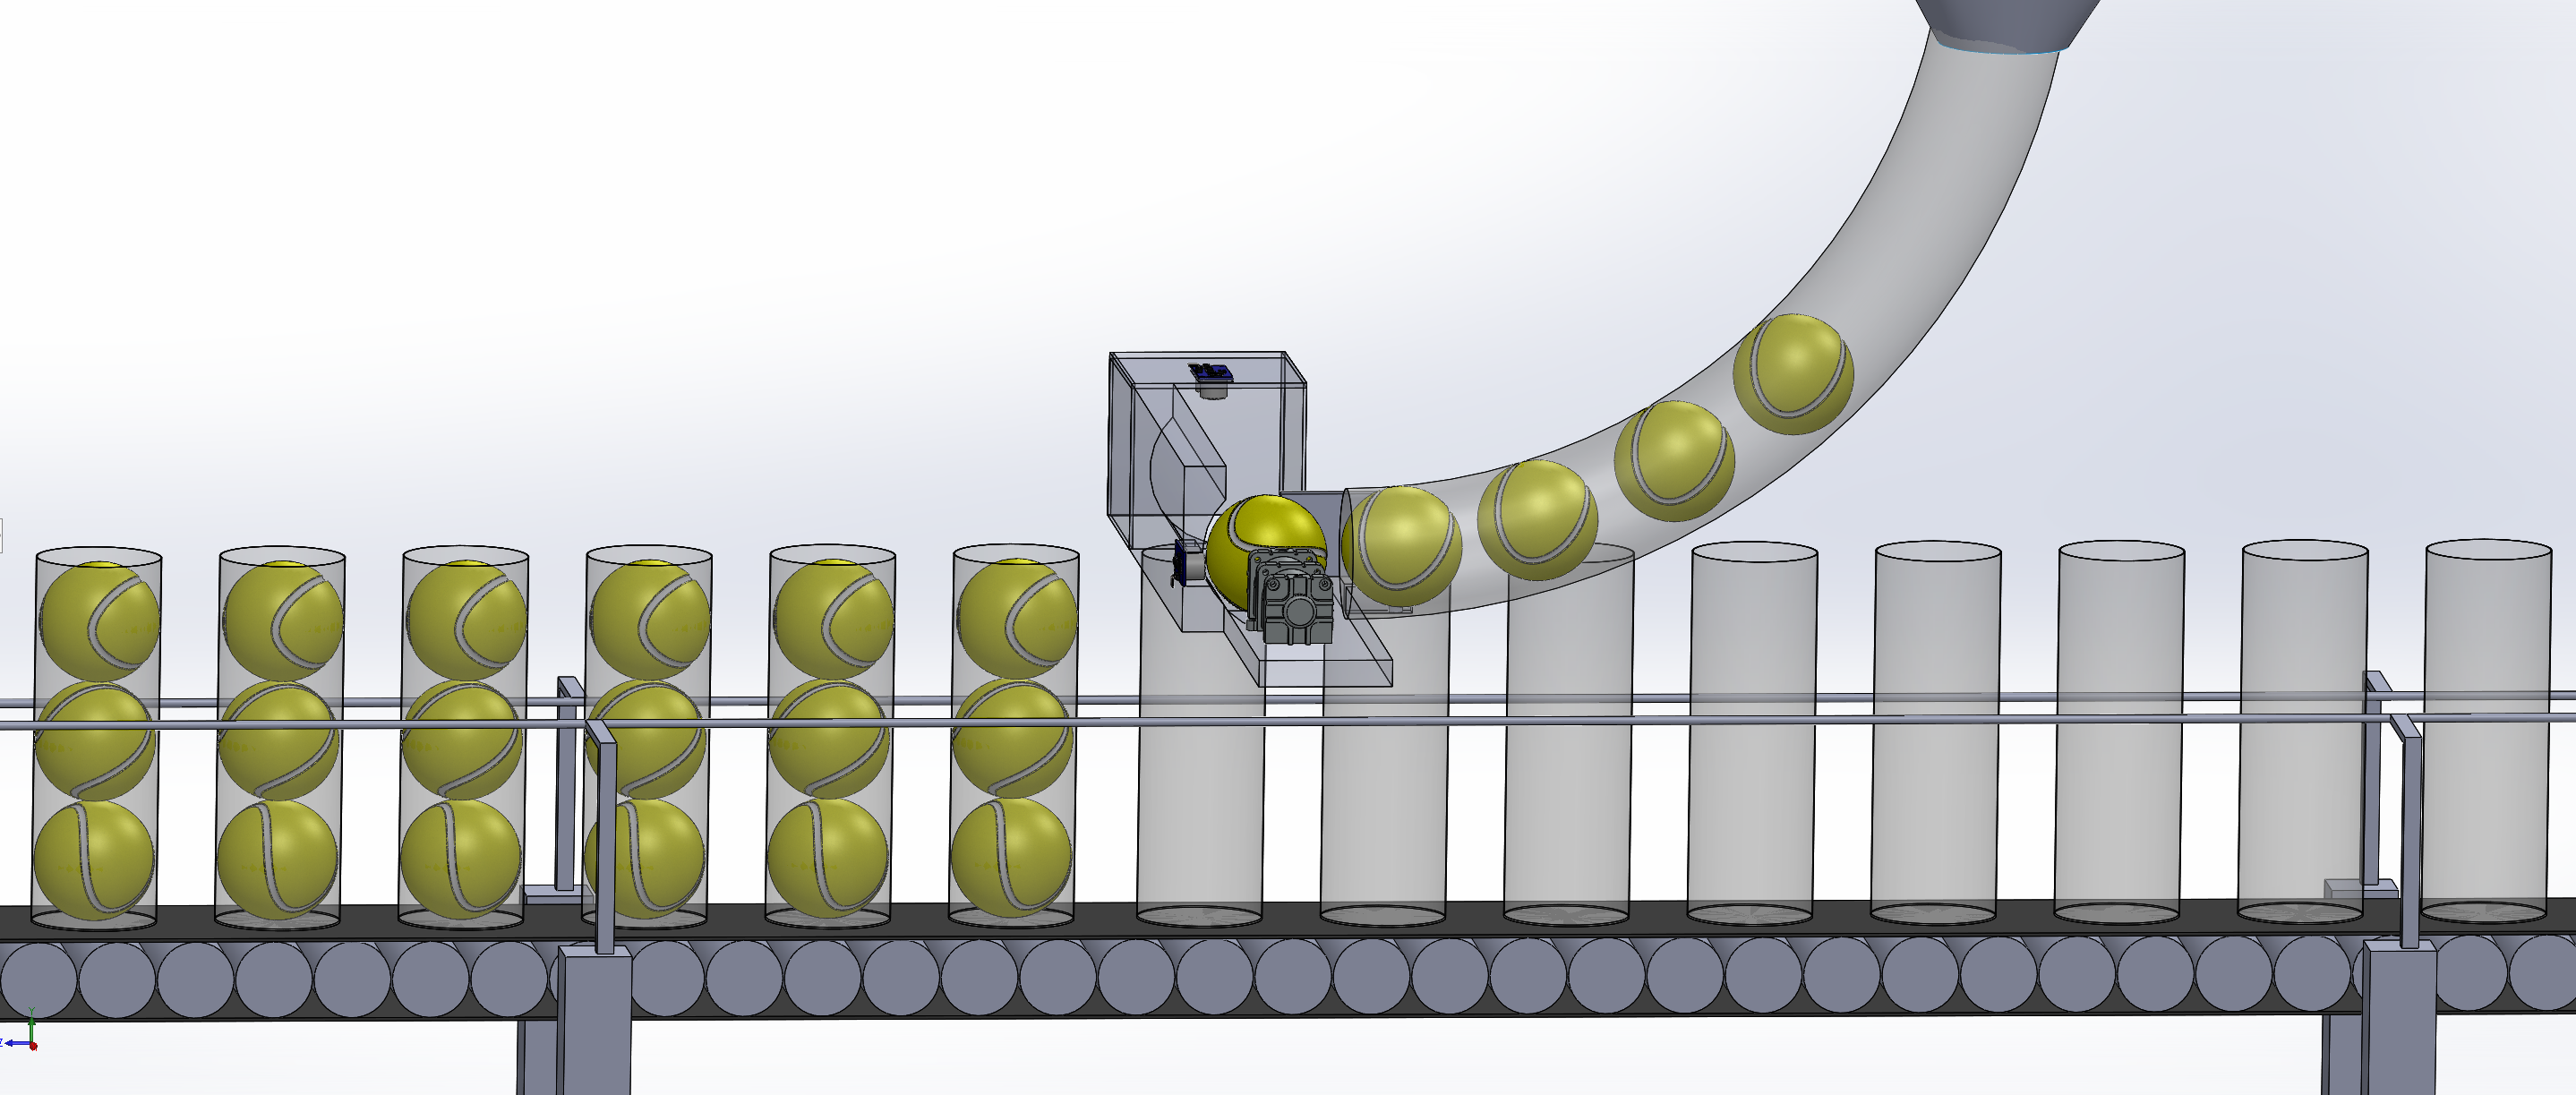
\includegraphics[width=7in]{./images/Line2}}
\caption{Overall System - Perspective\label{Line2}}
\end{figure*}

\begin{figure*}
\centerline{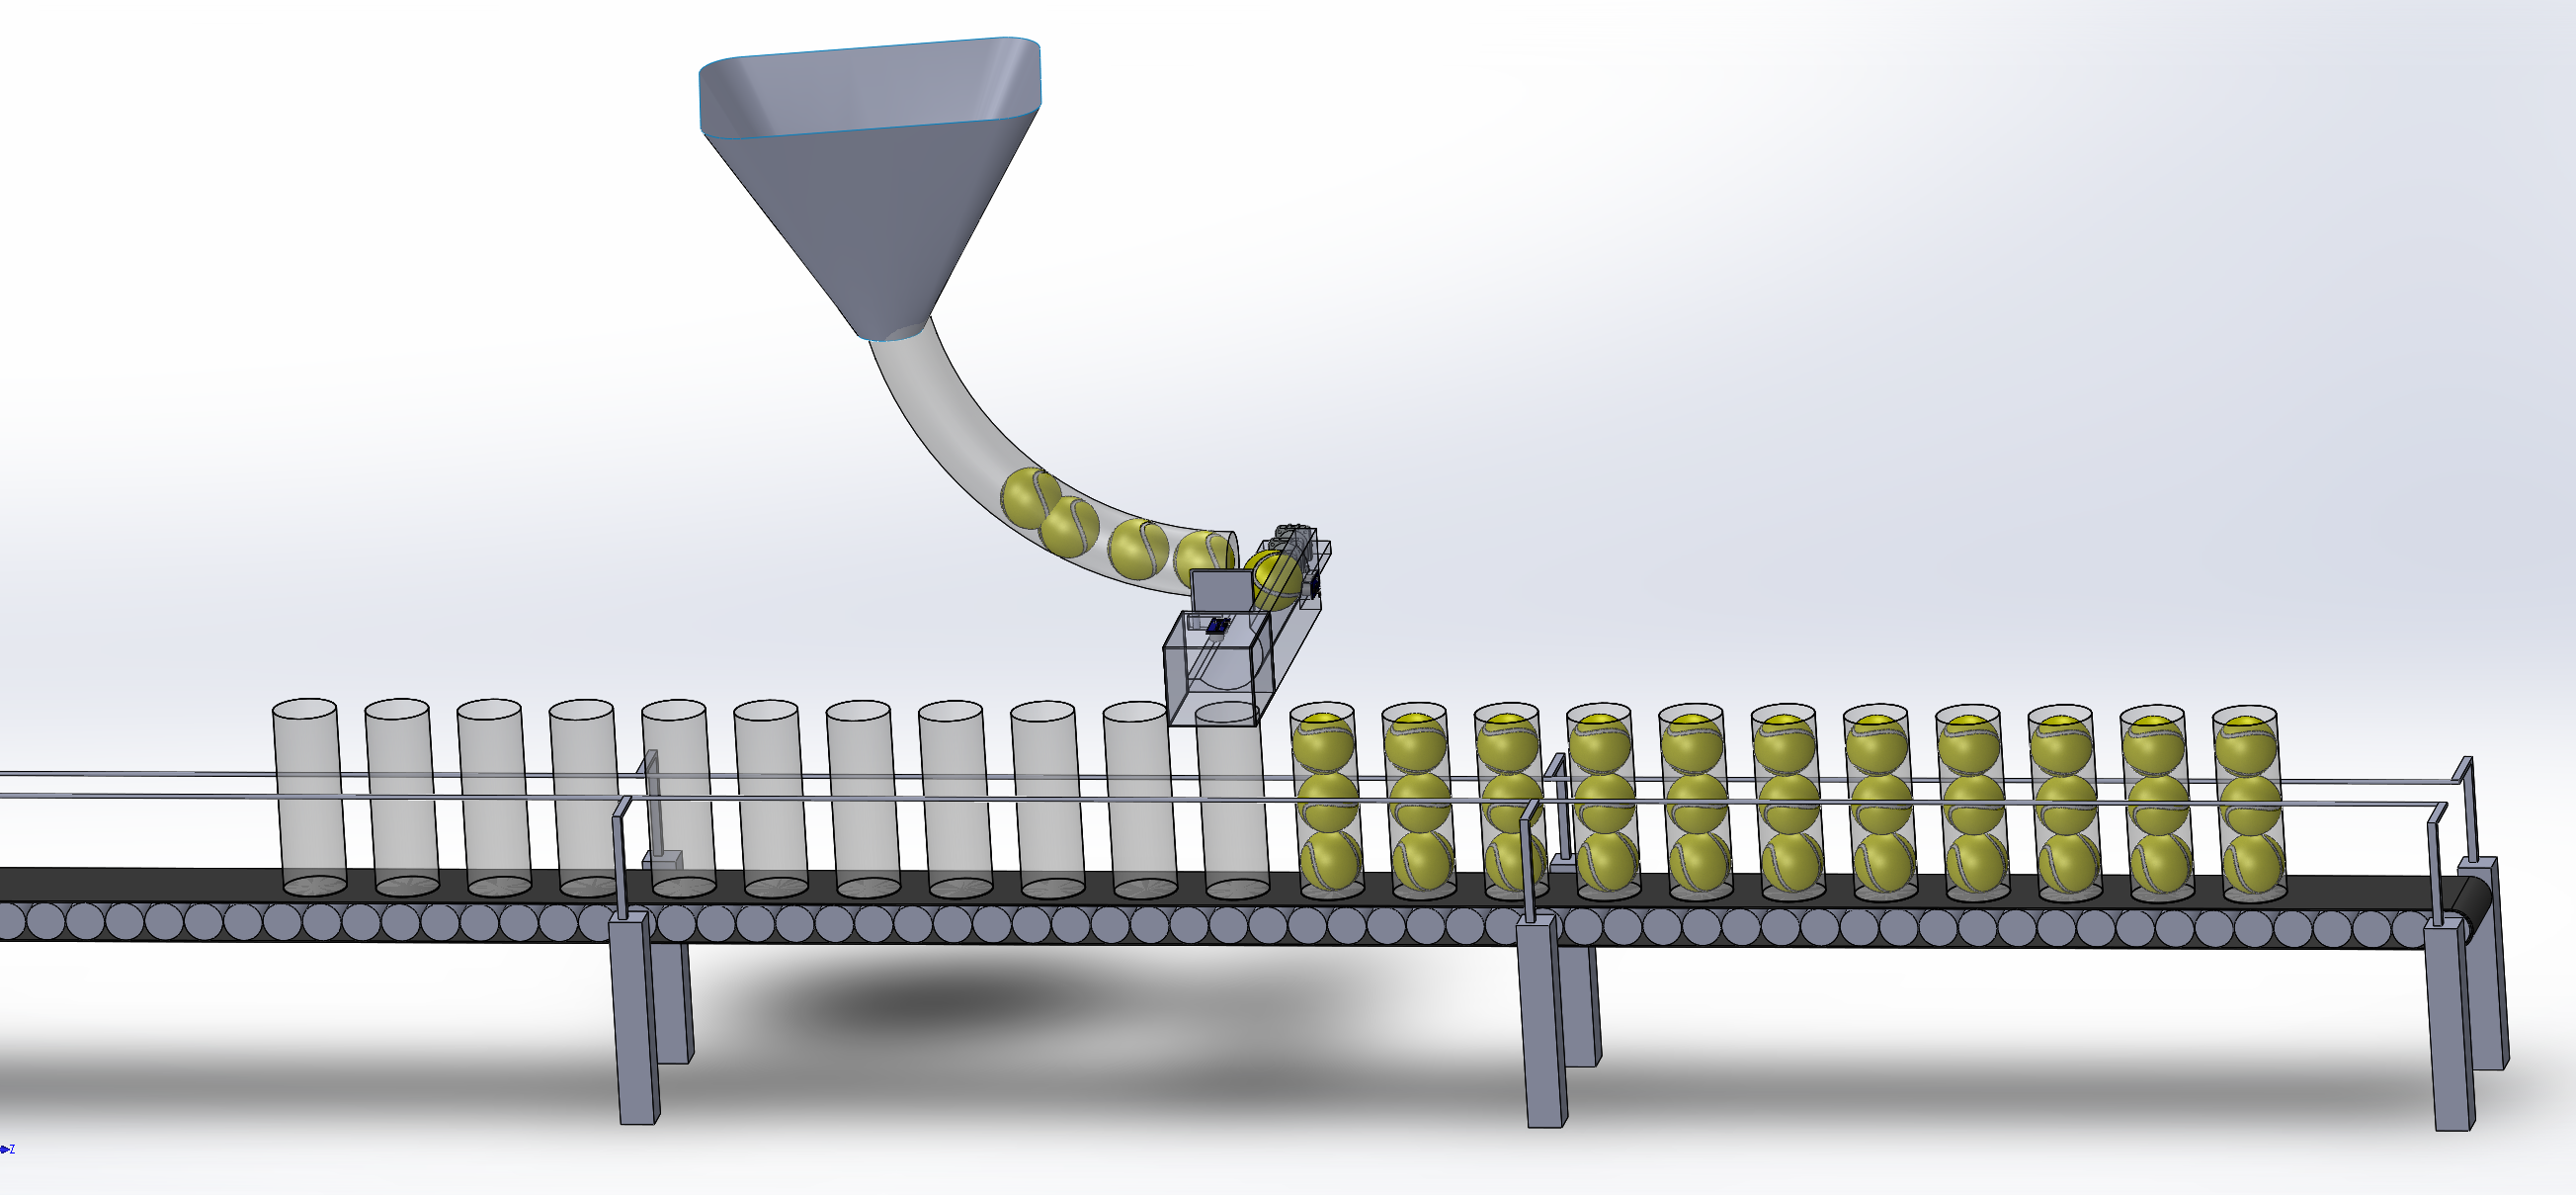
\includegraphics[width=7in]{./images/Line}}
\caption{Overall System\label{Line}}
\end{figure*}



\section{Results}


The results of the simulation are not ideal due to the many factors that have to be considered on a real project. The physical interaction of all the components have to be taken into consideration. All these factor can be seen on a real model and that's the idea behind a design process like this, where we round the intrinsic factors that are of minor importance in favour of having the big picture revealed and then measure and adjust the real product at the end.

Although, since the aim of the project was to practice the design process, it was fully achieved since an electrical, mechanical and software, therefore, mechatronic system was fully developed and integrated.


\section{Discussion and Conclusions}

In this project a electrical, mechanical and software system were developed and integrated, fulfilling the aims of the project. The performance of the project can only be measured but assessing the simulations, unfortunately the real implementation of the project is not possible at this moment. Although the knowledge of how to integrate the systems was of great value.

Improvements and recommendations for the project in future developments include the following, to name a few:

\begin{enumerate}
\item If the project were to be implemented, the first idea measure the real world performance and compare with the simulations.
\item The system can be improved by changing the LED's for a real motor and the solenoid valve on the electronic simulation.  
\item Use real parts Datasheets and a more robust simulator like Eagle
\item Another The use of counters to specify the amount of packs delivered and also a check system to count the amount of balls inside the package is of easy implementation using computer vision and tools like OpenCV.
\end{enumerate}






\clearpage
\newpage

\begin{thebibliography}{00}

\bibitem{ref1} A. Parr, \emph{Hydraulics and Pneumatics - A technician's and engineer's guide}, 2nd ed., Ed. Butterworth-Heinemann, Oxford - UK 1998.

\bibitem{ref2} W. Bolton, \emph{Mechatronics - Electronic control systems in mechanical and electrical engineering}. United Kingdom: Pearson Education Limited, 2019.

\bibitem{ref3} (Proteus wesite Online Help) Labcenter. (2020, May).  Available: https://www.labcenter.com/.

\bibitem{ref4} (16x2 LCD Module) Datasheet. (2020, May).  Available: https://components101.com/16x2-lcd-pinout-datasheet.


\bibitem{ref5} (Arduino Store)(2020, May). Available: https://store.arduino.cc/usa/arduino-uno-rev3. 

\bibitem{ref6} (Ultrasonic Sensors: Applications in the Internet of Things)(2020, May). Available: https://blog.seebo.com/iot-ultrasonic-sensors/

\end{thebibliography}

\clearpage
\newpage

\onecolumn

\appendix

\begin{lstlisting}[language=Python, caption=Arduino Programming]
#include "Ultrasonic.h"
#include <LiquidCrystal.h>

const int rs = 12, en = 11, d4 = 5, d5 = 4, d6 = 3, d7 = 2;
LiquidCrystal lcd(rs, en, d4, d5, d6, d7);

const int echoPin = 6; 
const int pingPin = 7; 
const int echoPin2 = 8; 
const int pingPin2 = 9; 
int led13 = 13;
int led10 = 10;

void setup() {
  lcd.begin(16, 2);

  pinMode(led13, OUTPUT);
  pinMode(led10, OUTPUT);
  
  pinMode(pingPin, OUTPUT); 
  pinMode(echoPin, INPUT); 
  pinMode(pingPin2, OUTPUT); 
  pinMode(echoPin2, INPUT); 
}

void loop() {
  long duration, duration2, cm, cm2;
  digitalWrite(pingPin, LOW);
  delayMicroseconds(2);
  digitalWrite(pingPin, HIGH);
  delayMicroseconds(10);
  digitalWrite(pingPin, LOW);
  duration = pulseIn(echoPin, HIGH);
  cm = microsecondsToCentimeters(duration); 

  digitalWrite(pingPin2, LOW);
  delayMicroseconds(2);
  digitalWrite(pingPin2, HIGH);
  delayMicroseconds(10);
  digitalWrite(pingPin2, LOW);
  duration2 = pulseIn(echoPin2, HIGH);
  cm2 = microsecondsToCentimeters(duration2); 

  lcd.setCursor(0, 0);
  lcd.print("UT cm: ");
  lcd.print(cm);
  lcd.setCursor(0, 1);
  lcd.print("UT cm2: ");
  lcd.print(cm2);
  
  if (cm < 20) {
    digitalWrite(led13, HIGH); 
    delay(1000);
    digitalWrite(led13, LOW);
  } else {
     digitalWrite(led13, LOW); 
  }
  
  if (cm2 < 6) {
    digitalWrite(led10, HIGH); 
    delay(1000);
    digitalWrite(led10, LOW);
    delay(1000);
  } else {
     digitalWrite(led10, LOW); 
  }
  delay(100); 
}

long microsecondsToCentimeters(long microseconds){
return microseconds / 29 / 2;
}
\end{lstlisting}


\end{document}
